\chapter{Arhitectura aplicaţiei}
\label{chapter:arh}

Proiectată privind către viitor, aplicaţia noastră oferă posibilitatea 
extinderii pe viitor în numeroase direcţii de dezvoltare. Am construit o 
platformă solidă pe baza căreia se poate dezvolta o aplicaţie CAD de un nivel 
comparabil cu a altor aplicaţii de acest tip.

Vom orienta prezentarea noastră în două direcţii. Întîi ne vom concentra asupra 
modelului de lucru. El reprezintă inima proiectului, un concept care uneşte în 
el toate capacităţile acestui proiect. Apoi vom trece la descrierea interfeţei 
cu utilizatorul, a cărei concepţie în sine prezintă o considerăm remarcabilă şi 
reprezintă o bază pentru dezvoltări ulterioare.

În Figura \ref{figure:arh} am făcut o reprezentare schematică a celor ce vor fi
enunţate mai jos, a structurii aplicaţiei şi a principalelor sale componente.

\begin{figure}[htp]
\begin{center}
  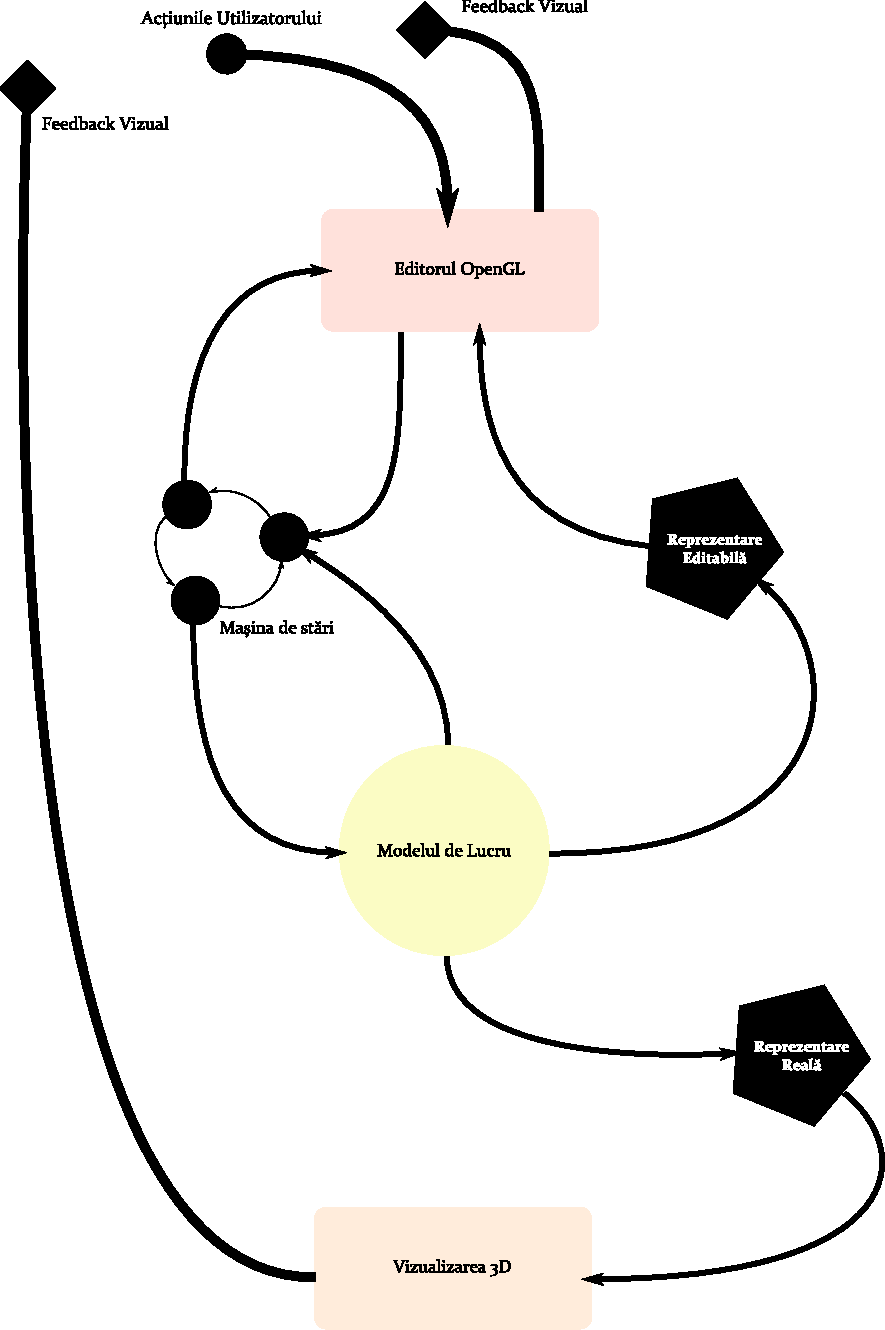
\includegraphics[width=\textwidth]{figures/arh-svg.pdf}
  \caption{Structura generală a proiectului \label{figure:arh}}
\end{center}
\end{figure}

\section{Modelul de lucru}

\begin{definition}
\label{define:model}
Numim \textbf{Model de lucru} reprezentarea într-o colecţie de obiecte Java a 
unei structuri arhitecturale ce poate fi modelată cu ajutorul acestui proiect.
\end{definition}

Modelul de lucru este o reprezentare a unei structuri pe care proiectantul 
doreşte să o reprezinte cu această unealtă într-o formă pe care programul o 
poate recunoaşte şi o poate reface cît mai fidel cu modelul real imaginat de 
proiectant.

\begin{definition}
\label{define:primitive}
Numim \textbf{Primitivă} unitatea structurală şi funcţională a Modelului de 
lucru. O primitivă poate fi o colecţie de alte primitive. De asemenea, o 
primitivă este un element ce poate fi materializat atît la nivel logic cît şi 
într-o reprezentare grafică.
\end{definition}

Primitivele sunt analogiile entităţilor logice în care un model real poate fi 
divizat pentru a-l reprezenta structurat. În seria de primitive ce pot apare în 
modelul logic pot exista primitive care nu au un analog imediat în lumea reală.

\begin{statement}
Modelul logic în totalitatea lui este o Primitivă.
\end{statement}

Plecînd de la aceste două noţiuni, vom încerca să prezentăm întreaga structură 
a Modelului de lucru şi modul în care acesta interacţionează cu aplicaţia în 
sine.

În esenţă, o primitivă este orice poate fi desenat. De aceea, la rîndul său 
modelul este o primitivă. Introducem două direcţii în care modelul poate fi 
reprezentat.

\begin{definition}
\label{define:realRender}
Numim \textbf{Reprezentare Reală} o materializare strictă în comenzi 
Java / OpenGL a unei reprezentări schematice tridimensionale a unei Primitive, 
realizată cu scopul formării unei imaginii asupra rezultatului final al 
construcţiei fizice a entităţii logice din spatele acelei primitive. 
\end{definition} Modelul tridimensional este deci cea mai apropiată formă de 
realitate pe care acest proiect o va reda pentru utilizatorii săi.

\begin{definition}
\label{define:editorRender}
Numim \textbf{Reprezentare Editabilă} o materializare strictă în comenzi 
Java / OpenGL a unei reprezentări schematice bidimensionale a unei Primitive, 
realizată cu scopul identificării vizuale a primitivelor şi accesării facilă 
prin intermediul unui editor a proprietăţilor primitivelor.
\end{definition}

Reprezentarea Editabilă este apropiată ca raţiune figurilor din desenul tehnic, 
şi de aceea identitatea lor vizuală este la rîndul ei asemănătoare acelor 
figuri. Alegerea acestor noţiuni este în strictă corelaţie cu detaliile de 
implementare ale aplicaţiei, care le vom detalia în următorul capitol. Pentru a 
ne face o idee despre cum aceste două reprezentări se potrivesc peste model, 
vom spune că reprezentarea modelului de lucru este juxtapunerea tuturor 
reprezentărilor celorlalte primitive existente în model, în ambele 
reprezentări. Desigur, asta implică că modelul în sine nu este decît un simplu 
container logic pentru toate celelalte componente ale aplicaţiei.

\subsection{Tipuri de primitive}
\label{section:primitives}
Alegerea setului de primitive de care va dispune această aplicaţie a fost o 
sarcină dificilă. Timpul de implementare este în directă corelaţie cu volumul 
de primitive care trebuiesc implementate.

Vom lăsa ca un exerciţiu viitor adăugarea de noi primitive care ar fi de un 
real ajutor utilizatorului acestei aplicaţii. Setul ales este considerat de 
autor ca fiind suficient pentru a oferi un set de funcţionalităţi de bază 
utilizabile pentru această aplicaţie şi destul de variate pentru a scoate în 
evidenţă potenţialul de creştere al acestui proiect.

\subsubsection{Ziduri şi Colţuri de Ziduri}

Elementele constructive esenţiale ale unei structuri sunt zidurile. Ele 
delimitează forma şi suprafaţa construcţiei, avînd un impact crucial asupra 
preţului de construcţie şi facilităţile ce vor putea fi oferite de acea 
construcţie.

Colţurile sunt un tip de primitivă indirect disponibilă proiectantului. Unirea 
capetelor a două ziduri se poate face printr-un colţ, care introduce de fapt o 
legătură permanentă între marginile acelor două ziduri. Constrîngerea este una 
punctuală, zidurile putînd avea orice orientare în cadrul modelului atîta timp 
cît sunt conectate la un colţ. Colţurile pot fi privite ca nişte puncte într-un 
plan.

Orice zid este conectat la două colţuri, \textbf{Colţul de Start} şi 
\textbf{Colţul de Stop}. Astfel poziţionat, lungimea şi orientarea unui zid 
este dictată de poziţia celor două colţuri. Astfel, un zid poate fi privit ca 
un segment ce leagă oricare două puncte (colţuri) dintr-un plan.

\subsubsection{Caracteristici de Ziduri}

\begin{definition}
\label{define:feature}
Numim \textbf{Caracteristică a unui Zid} orice Primitivă ce este asociată în 
mod direct cu un zid.
\end{definition}

Toate Caractersticile sunt constrînse poziţional în lungimea zidului. Ele 
adaugă elemente suplimentare modelului care sunt strict legate în realitate de 
existenţa unui zid. Exemple tipice de caracterstici ce elucidează şi mai bine 
ce reprezintă o caracteristică ar fi:

\begin{itemize}
  \item Fereastră
  \item Uşă
  \item Deschidere -- orice trecere completă prin volumul unui zid (o intrare 
  fără uşă, sau deschiderea unei ferestre fără o fereastră montată în ea)
  \item Cavitate -- orice intrare parţială în volumul unui zid, ca un raft 
  interior într-un perete fals.
  \item Ingroşăre -- orice adăugare la volumul unui zid, o îngroşare într-o 
  anumită zonă, ce poate servi, prin analogie, ca un raft exterior într-un 
  perete.
\end{itemize}
  
\subsubsection{Decoraţiuni}
  
\begin{definition}
\label{define:decoration}
\textbf{Decoraţiunile} sunt Primitive care nu au legătură strictă cu structura 
construită, însă oferă un plus de realism şi poate sugera viitoarea destinaţie 
a diferitelor spaţii din model.
\end{definition}
  
\begin{itemize}
  \item Canapea
  \item Masă
  \item Toaletă
  \item Chiuvetă de baie
  \item Vană
  \item Chiuvetă de bucătărie
  \item Aragaz
  \item Frigider
  \item Masă de bucătărie
\end{itemize}

Dintre aceste Decoraţiuni, unele dintre ele vor fi implementate ca şi 
Caracterstici, datorită constrîngerii lor reale de a apărea pe un zid. Dintre 
cele menţionate mai sus, dăm exemplu chiuveta care întotdeauna apare în 
vecinătatea unui perete.

În Figura \ref{figure:model-arh} vom sumariza cele prezentate mai sus printr-o 
diagramă cu toate componentele modelului de lucru.

\begin{figure}[htp]
\begin{center} 
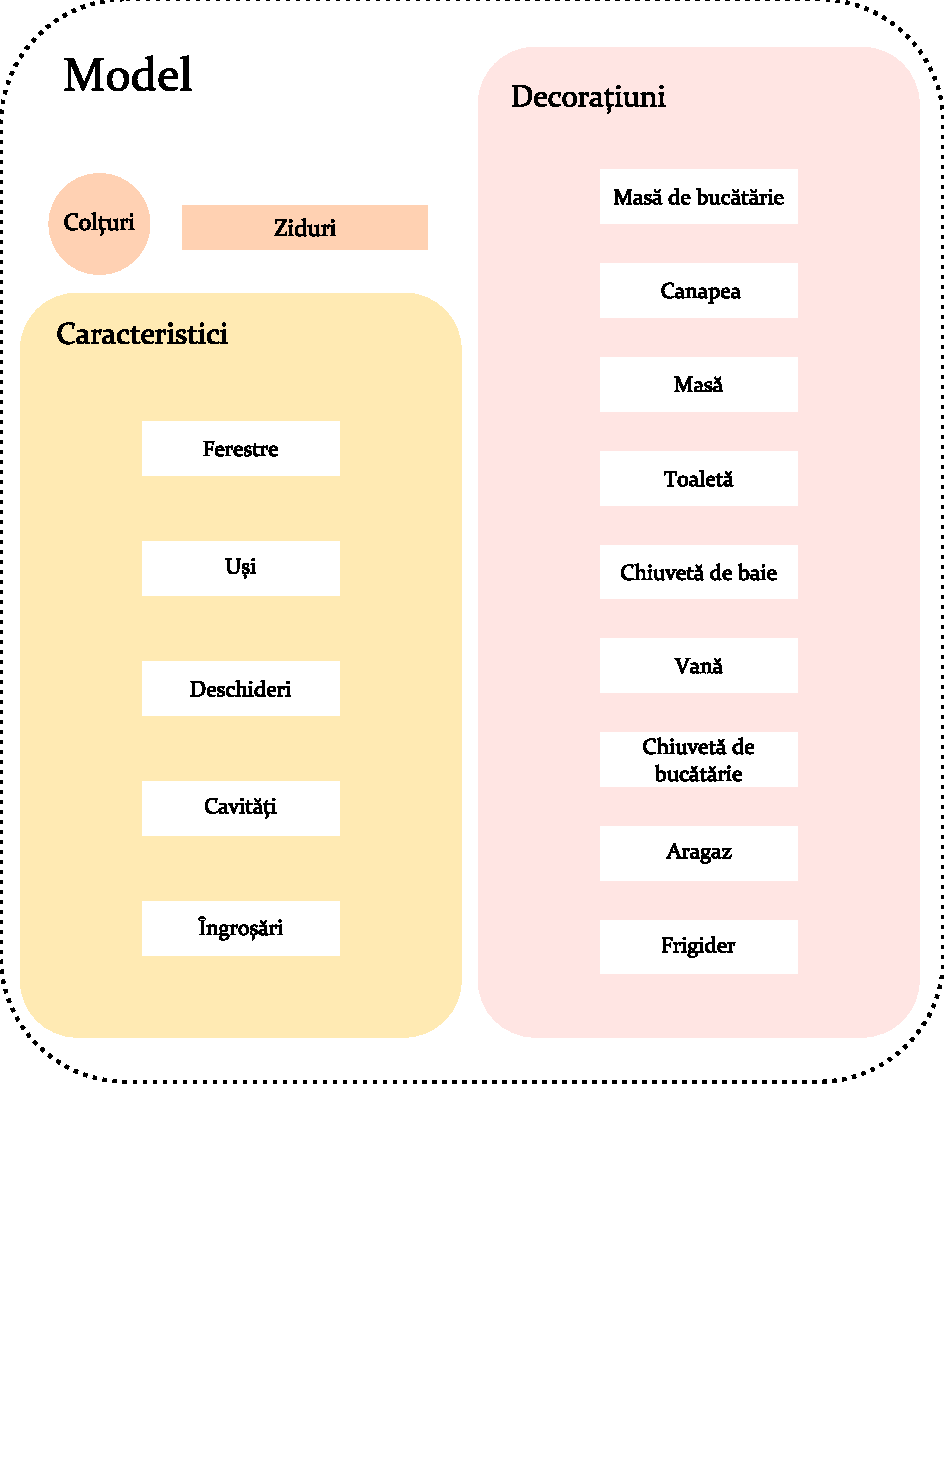
\includegraphics[width=\textwidth]{figures/drawing.pdf} \caption{Arhitectura 
Modelului de Lucru}
  \label{figure:model-arh}
\end{center}
\end{figure}

\subsection{Aspecte ale modelului}

\begin{definition}
\label{define:model-aspect}
Numim \textbf{Aspect al Modelului de Lucru} orice formă de interpretare a unei 
primitive aflate într-un model de lucru care nu are legătură cu modelul şi 
structura sa, dar ajută alte componente ale aplicaţiei în a interacţiona cu 
acesta.
\end{definition}

Pentru modelarea funcţionalităţii editorului, orice Primitivă 
(\ref{define:primitive}) este considerată ca un element ce poate fi desenat 
într-un editor. Fiecare Primitivă trebuie să specifice modul în care ea urmează 
să fie desenată în spaţiul bidimensional al editorului.

Unele primitive sunt desenate direct de către model, altele, cum ar fi 
Caracteristicile (\ref{define:feature}), ale căror desenare intră în 
sarcina zidului din care fac parte.

Acest aspect al modelului reprezintă materializarea \textbf{Reprezentării 
Editabile} (\ref{define:editorRender}).

Un alt aspect adăugat modelului este \textbf{Selectabilitate}.

\begin{definition}
\label{define:selectable}
Orice Primitivă care din punct de vedere al interfeţei editorului poate fi 
selectat prin diverse metode de utilizator se spune că este 
\textbf{selectabilă}, sau că are un aspect de \textbf{Selectabilitate}.
\end{definition}

Primitivele pot reacţiona la schimbarea stării lor de selectabilitate şi la 
rîndul său editorul poate trata evenimentul schimbării selecţiei în funcţie de 
implementarea dorită.

În fine, ultimul aspect al modelului necesar implementării editorului este cel 
de \textbf{Navigabilitate}.

\begin{definition}
\label{define:hoverable}
În momentul în care mausul trece deasupra unei 
astfel de componente, ea poate reacţiona prin evenimente implementate la 
nivelul editorului, avînd astfel aspectul de \textbf{Navigabilitate}.
\end{definition}

Multe Primitive folosesc această proprietate pentru a-şi schimba starea de 
selectare. Fiecare Primitivă selectabilă defineşte o stare proprie în care
editorul va trece în momentul în care primitiva respectivă este selectată. Dacă
primitiva nu defineşte o astfel de stare, atunci editorul rămîne în starea de
navigare.


\section{Editorul OpenGL}
\label{section:opengl-editor}

Înainte de a fi un editor pentru Modelul de Lucru (\ref{define:model}), 
editorul OpenGL dezvoltat de noi este un punct de plecare foarte bun pentru 
orice editor care necesită folosirea facilităţilor OpenGL. Vom încerca să 
descriem succint arhitectura editorului, evidenţiind caracteristicile generice 
cît şi particularizările de suprafaţă care au fost necesare pentru integrarea 
cu funcţionarea dorită.

Editorul este în principiu o suprafaţă de desenare OpenGL cu aspect 
bidimensional ce poate interacţiona cu utilizatorul prin intermediul interfeţei 
oferite de RCP, adică evenimentele ale mausului, ale tastaturii, ale 
vizualizărilor de structură şi de proprietăţi, despre care vom aminti mai jos.


\subsection{Editorul ca maşină de stări}

Editorul OpenGL funcţionează ca o maşină de stări. Editorul suportă 
înregistrarea stărilor noi şi controlează viaţa tuturor stărilor înregistrate 
în stiva sa de stări.

La un moment dat o singură stare este activă. O stare activă poate controla 
toate evenimentele pe care le primeşte editorul şi poate să introducă noi stări 
în stivă sau să modifice modelul în funcţie de evenimentele care au avut loc. 
Starea decide cînd viaţa ei a luat sfîrşit. Această decizie este comunicată 
editorului care apoi deînregistrează starea din stivă.

În Tabela \ref{table:editor-states} vom prezenta ciclul de viaţă al unei stări. 
Acest model de ciclu de viaţă a fost stabilit în funcţie de necesităţile 
editorului OpenGL, pentru a-i permite acestuia să interacţioneze sincron cu 
schimbările de stare ce pot fi controlate asincron de către evenimentele 
aplicaţiei.

Dintr-o anumită privinţă, acest ciclu de stare poate fi privit ca o serie de 
meta-stări ale aplicaţiei (i.e. stări ale stărilor).

\begin{table}[htp] \caption{Ciclul de viaţă al stărilor Editorului OpenGL
\label{table:editor-states}}
\begin{tabular}{|\col{0.23}|\col{0.73}|}

\hline FRESH & La construcţia unei stări ciclul de viaţă este setat în poziţia 
FRESH. Editorul va citi orice stare setată pe acest mod şi o va seta ca şi 
stare activă, înregistrînd toate rutinele de tratare a evenimentelor pentru 
această stare în cadrul editorului. Starea curentă este setată ca activă şi 
modul ei este trecut în RUNNING. Starea activă anterioară este trecută pe modul 
SLEEPING. \\

\hline RUNNING & După ce editorul iniţializează o stare, ea este în modul 
RUNNING. În acest mod starea primeşte toate evenimentele editorului. Decizia de 
a părăsi această stare se poate lua după două criterii. a) La discreţia stării 
în sine, prin trecerea în modul TERMINATED sau b) la discreţia editorului, în 
momentul sosirii unei noi stări FRESH, cînd starea curentă trece în SLEEPING. \\

\hline SLEEPING & Toate stările care au fost oprite de editor la apariţia unei 
stări noi se adună într-o stivă şi modul lor este trecut în SLEEPING. Ele pot 
sta în acest mod un timp nedefinit şi pot să nu-l părăsească niciodată. Ele pot 
reveni la starea RUNNING în momentul în care se află la vîrful stivei şi starea 
activă trece în modul TERMINATED. Atunci editorul automat va muta starea din 
capul stivei ca stare activă şi ea va deveni RUNNING. De aceea rutina de 
tratare a tranziţiei în RUNNING cît şi rutina de tratare în starea TERMINATED 
trebuie să aibă în vedere posibilitatea rulării de mai multe ori pentru aceeaşi 
stare (i.e. să nu trateze iniţializări, care se fac în mod normal în starea 
FRESH) \\

\hline TERMINATED & Odată ce starea consideră că şi-a încheiat activitatea, ea 
poate alege să treacă în modul TERMINATED. Odată ajunsă în acest mod, starea va 
fi deînregistrată din lista de captare a evenimentelor editorului şi va fi 
scoasă permanent din lista stărilor editorului.\\

\hline
\end{tabular}
\end{table}

Stările editorului sunt folosite pentru a manipula modelul de lucru. Ele pot 
adăuga şterge sau schimba diverse proprietăţi ale primitivelor aflate în model. 
Din acest motiv, stările sunt strict asociate cu diversele tipuri de primitive 
din model.

Există o stare nativă a editorului, anume starea de navigare. Este singura stare
definită aici care nu se termină niciodată, şi este pornită automat de către
editor la iniţializarea sa. Starea de navigare este responsabilă de
administrarea diverselor proprietăţi ale obiectelor, ea fiind cea care ia
decizia -- şi în acelaşi timp informează -- fiecare proprietate de starea sa de
acoperire cu mausul. De asemenea, ea porneşte mecanismul de selecate a
obiectelor şi de trecere în starea predefinită de fiecare obiect care poate fi
selectat dintr-o scenă.

Starea de selectare este o stare specială în care editorul trece atunci cînd un
obiect este selectat cu ajutorul diverselor metode puse la dispoziţie de Eclipse
RCP. Starea de selectare este folosită de Colţuri, spre exemplu, pentru a iniţia
procedura de transformare prin deplasare a mausului, mişcare prin care poziţia
Colţului este modificată. Starea de selecţie a colţului trebuie să aibă în
vedere -- precum toate celelalte stări de selecţie -- că selecţia poate avea mai
multe surse şi comportamentul său predefinit -- de a transporta cu ajutorul
mausului colţul -- nu este valid decît in cazul selecţiei cu ajutorul mausului.
Această discriminare se face cu ajutorul stării de acoperire cu mausul a
Colţului respectiv\footnote{Dacă mausul nu este deasupra componentei, înseamnă
că selecţia avut loc prin alte mecanisme, şi atunci se anulează procedura de
mutare a colţului}.

\subsection{Capacităţi asincrone}

Editorul OpenGL este optimizat pentru motorul asincron de sincronizare, 
desenare şi tratare a evenimentelor ale aplicaţiilor Eclipse RCP. Deşi vom 
intra în detalii în capitolul \ref{chapter:impl}, amintim doar aici că într-o 
singură aplicaţie se pot edita oricîte Modele de Lucru, fără nici un impact 
asupra unuia dintre ele şi fără interferenţe de nici un fel atît în logica 
modelului cît şi în ciclul de randare.

\section{Vizualizarea 3D OpenGL}
\label{section:view}

După cum am văzut în secţiunea \ref{section:opengl-editor}, Editorul OpenGL 
serveşte la manipularea Modelului de Lucru (\ref{define:model}) şi a 
proprietăţilor diverselor Primitive (\ref{define:primitive}) din acest Model. 
Sarcina vizualizării tridimensionale a modelului cade în măinile componentei 
despre care vom discuta în această secţiune.

Diferenţa principală dintre Editor şi Vizualizare este că cea din urmă nu 
permite interacţiunea cu proprietăţile modelului, ci doar proiecţia lor într-o 
lume tridimensională. Proiecţia se face într-o scenă văzută în perspectivă şi 
cu toate obiectele desenate prin contur cu muchiile din spate ascunse. Modelul 
poate fi explorat cu ajutorul mausului, însă nu se poate interacţiona în nici 
un fel similar cu capacităţile editorului.

\subsection{Aspectul de desenare reală}

La rîndul său, Vizualizarea 3D introduce un aspect (\ref{define:model-aspect}) 
asupra Modelului de Lucru. Acest aspect este cel de \textbf{desenare reală}. 
Deşi structura ierhahică a liniei de randare este similară cu cea a aspectului 
de randare pentru editare, există o singură diferenţă semnificativă.

Pentru randarea scenei cu contur ascunzînd muchiile din spate, OpenGL necesită 
ca scena să fie randată în două treceri. Prima trecere reprezintă volumele de 
randare şi în a doua trecere se desenează contururile.

În principiu, aspectul de desenare reală trebuie să aibă în vedere optimizarea 
celor două treceri pentru a obţine doar acele contururi care sunt de interes 
pentru utilizator, fără a marca toate poligoanele din scenă.

\subsection{Conexiunea cu Editorul OpenGL}

Precum Editorul OpenGL, Vizualizarea 3D OpenGL are şi ea ample capacităţi 
asincrone, răspunzînd la solicitările editorului şi putînd servi simultan 
nevoile a mai multor editoare. Platforma RCP forţează ca orice vizualizare să 
existe o singură dată în interfaţa grafică. Prin această limitare se impune ca 
Vizualizarea 3D să reprezinte doar modelul aflat în Editorul activ la un moment 
dat.

De asemenea, Vizualizarea 3D are capacitatea de a reprezenta orice modificare
are loc în Modelul de Lucru în timp real, în momentul în care datele parţiale
sunt salvate în Model.

\section{Vizualizarea structurii modelului}

Eclipse RCP oferă o vizualizare predefinită pentru descrierea structurii 
conţinutului unui editor\footnote{cunoscută în documentaţia Eclipse ca 
\textit{Content Outline View}}. În cazul de faţă, conţinutul logic al 
editorului îl reprezintă tocmai modelul, şi astfel o reprezentare a structurii 
modelului a fost furnizată pentru această vizualizare.

În cadrul acestei vizualizări utilizatorul poate modifica selecţia curentă în
editor şi poate afla informaţii despre poziţia diverselor componente ale
modelului. Afişarea acestor informaţii este în strictă legătură cu sursa de
selecţie.

\section{Sursa de selecţie. Descriptorul de conţinut}

Orice Pagină Eclipse\footnote{Paginile sunt descrise în Secţiunea
\ref{section:workbench}} poate avea o sursă de selecţie. O sursă de selecţie
este un concept abstract care vine asupra conţinutului unui editor pentru a
ajuta sincronizarea afişării informaţiilor în diverse vizualizări care sunt
implementate în program.

Special pentru scopurile Vizualizării 3D şi a Vizualizării de structură despre
care amintim acum, am definit o sursă de selecţie strict legată de modelul de
lucru din editor.

Această sursă de selecţie implementează conceptul abstract definit în Eclipse şi
îl adaptează nevoilor modelului nostru. El este capabil şi conştient de
diversele tipuri de Primitive care există în model şi poate distinge între
stările acestora.

Acesta reprezintă deci un descriptor de conţinut al editorului care este folosit
de către Pagina Eclipse pentru sincronizarea diverselor componente ale
interfeţei grafice.
